
\begin{dialog}{一位烟民富于启发性的思想}

\begin{quote}
阿基里斯应邀来到螃蟹的家里。
\end{quote}

\begin{dialogue}

\item[阿基里斯]我发现比我上次来这儿时你又添了些新东西,老蟹。你那幅新弄到的画尤其引人注目。

\item[螃蟹]谢谢。有些画家我很喜欢——特别是雷内·马格里特。我所拥有的画中大部分都是他作的。他是最对我口味的艺术家。

\item[阿基里斯]我得说它们的造形都挺有趣。马格里特的这些画中有许多地方都使我想起最对我口味的画家艾舍尔的作品。

\item[螃蟹]这一点我也能看得出来。马格里特和艾舍尔在表现悖理的和虚幻的世界时,都运用十分写实的手法,两个人在运用视觉形象以唤起观众的情感方面都具有很准确的感觉能力,而且——他们作品的爱好者们常常忽视这一点,就是他们都具有对优美线条的感受力。

\item[阿基里斯]不过,他们彼此之间还是有很大不同的。我不知道怎么描述这种区别。

\item[螃蟹]细致入微地比较这两个人一定非常引人入胜。

\item[阿基里斯]我认为,马格里特对现实的把握是惊人的。比如那儿挂着的那幅画吧,画面上有一棵树,树后面还有一支巨大的烟斗,画得太迷人了。

\begin{figure}
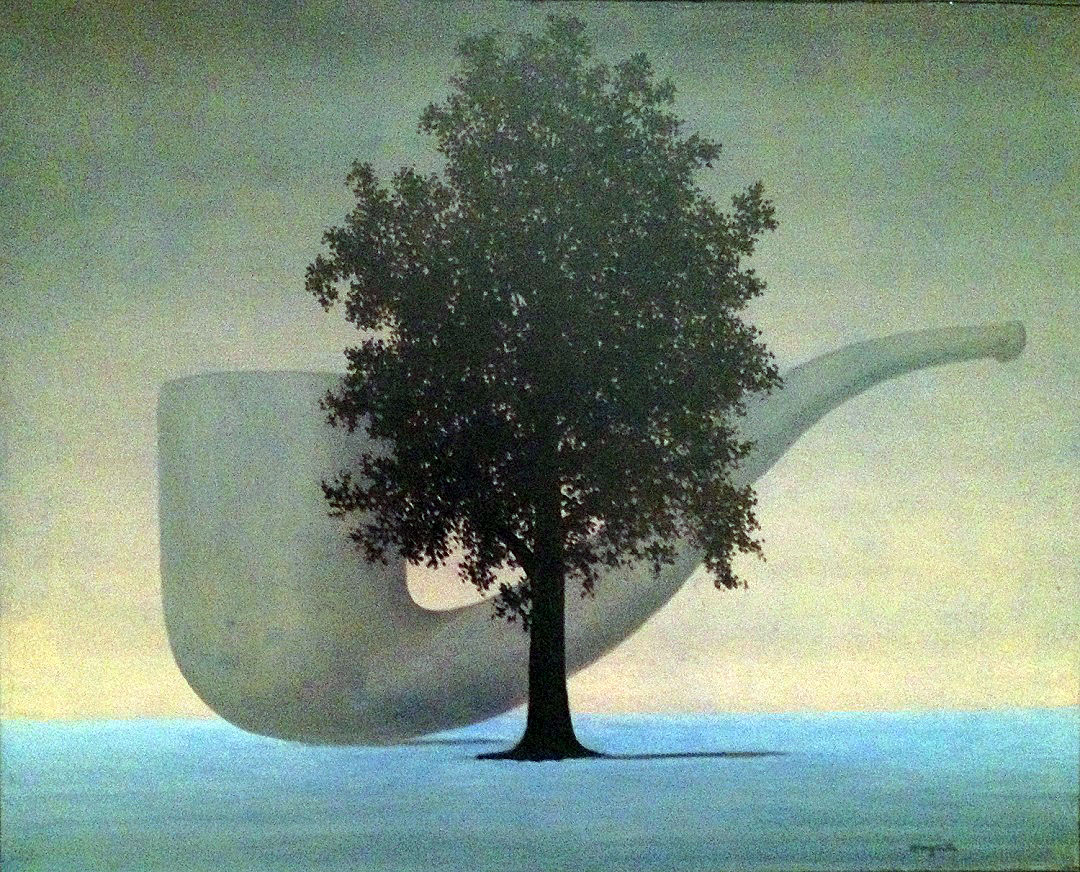
\includegraphics{img_077.jpg}
\caption[影子,马格里特作。]
  {影子,马格里特作(1966)。}
\end{figure}

\item[螃蟹]你是想说一只大小正常的烟斗和它前面的一棵微型树吗?

\item[阿基里斯]哦,是这样,我看错了?嗯,不管怎么说,我第一眼看见它时,就觉得闻到了烟斗发出的烟味儿!你想象得出我有多荒唐吗?

\item[螃蟹]我能理解。我的客人们经常被它骗住了。

\dnote{(他一边说着,一边过去伸手把画中的烟斗从树后拿出,然后翻过来,在桌上磕了磕,房间里马上充满了烟味儿。他开始往里面装新的烟丝。)}

这是只很不错的旧烟斗,阿基。信不信由你,我总爱往烟丝里掺点稻草,这样抽起来味道更好。

\item[阿基里斯]掺稻草!真的吗!

\item[螃蟹]\dlnote{(拿出一盒火柴,点上烟斗)}你想尝尝吗,阿基?

\item[阿基里斯]不,谢谢。我只是偶尔吸吸雪茄。

\item[螃蟹]没问题!雪茄我这儿也有!\dlnote{(把手伸向马格里特的另一幅画,画面上一辆自行车放在一支点燃的雪茄上。)}

\begin{figure}
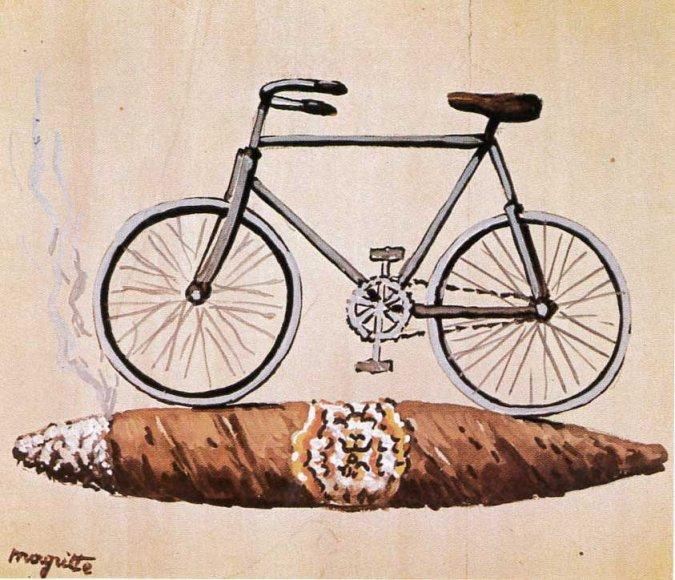
\includegraphics{img_078.jpg}
\caption[优雅状态,马格里特作。]
  {优雅状态,马格里特作(1959)。}
\end{figure}

\item[阿基里斯]噢——不,谢谢,现在还不想抽。

\item[螃蟹]你随便。我这人可是个不可救药的烟鬼。这倒叫我想起来——你无疑知道老巴赫有用烟斗吸烟的嗜好?

\item[阿基里斯]我想不大起来了。

\item[螃蟹]老巴赫喜欢作诗、玄想、吸烟,还喜欢作曲演奏(当然喜好程度不一定是这么个顺序)。他把这四者弄进一首不太高明的诗里,然后还为它谱了曲。这写在他为妻子安娜·马达莱娜所保存的那本著名的音乐笔记本里,它的题目是
\begin{center}\kaishu\large
一位烟民富于启发性的思想\note{巴赫此诗的英译引自大卫和曼德尔的《巴赫读本》,第97--98页。}
\end{center}
\nopagebreak
\begin{verse}
我拿起烟斗装满叶烟,\\
吞云吐雾以消磨时间,
人在那儿坐着,却溜走了思想——\\
它飘向一幅图画,晦黯而忧伤:\\[1]
那画告诉我这是多么相像:\\[1]
我和这烟斗简直就是一样。
\medskip
这喷香溢郁的烟斗同我相仿,\\
都不过是尘芥,不过是土壤;
我最终也要归为尘灰。\\
烟斗落地,没等听到声响,\\[1]
就已经拦腰摔断,不幸遭殃;\\[1]
相同的命运我也将承当。
\medskip
洁白的烟斗没有污斑,\\
从未玷染,从未弄脏。
可总有一天会命归无常,\\
在草地下掩埋这副皮囊;\\[1]
我的肉体将变黑,一副腌\textcombine{卧龙}相,\\[1]
就像这烟斗,若是它使用得经常。
\medskip
当烟斗被点燃,闪耀着火光,\\
瞧,它们立刻就冒出青烟袅袅飘荡;
轻烟散进空气,无处寻访,\\
烟斗里便只剩有灰烬留藏。\\[1]
虚名也将消泯,正同那青烟一样,\\[1]
而躯体最终只不过化作土壤。
\medskip
吸烟时这种事也发生得经常:\\
架上的塞烟器不翼而飞,给你添忙,
这下你只好上手,虽然不很便当,\\
可手指伸进烟锅,难免要被烫伤。\\[1]
既然烟斗里都有痛苦伏藏,\\[1]
地狱里的痛苦将会何其难当!
\medskip
由对烟斗的沉思,导向了别的玄想,\\
沉溺在格致冥思中,
也有益于身心的健康;\\
这样吞云吐雾,心中着实舒畅,\\[1]
因此无论在国内、国外、在陆地或海洋,\\[1]
我都要一边抽我的烟斗,\\[1]
一边坚定对上帝的信仰。
\end{verse}
这种哲学倒是满有意思的,不是吗?

\item[阿基里斯]的确是。老巴赫是舞文弄墨的一把好手。

\item[螃蟹]你正好说出了我要说的话。其实我这辈子也曾写过一些打油诗,可我担心我的诗鄙陋不中雅听。我没有这种遣词炼句的本领。

\item[阿基里斯]哦,哪里,老蟹。你——我怎么说呢——论俏皮、戏谑样样都有。要是你能给我唱一支你的歌,老蟹,我将感到不胜荣幸。

\item[螃蟹]太抬举我了。我给你放一张我的唱片怎么样?我记不得它是什么时候灌制的了。歌的名字是“云俦梅友”。

\item[阿基里斯]太有诗味了!是首山水诗吧?

\dnote{(螃蟹从他的架子上拿下一张唱片,走到一架庞大而复杂的机器面前,把它打开之后,将唱片放入一个看上去怪吓人的机械嘴里。突然,一道绿色的亮光扫过唱片的表面,过了一会儿,那唱片就悄没声地闪进那架古怪机器的肚子里的什么地方去了。又过了一会,才传出了螃蟹的歌声。)}

\begin{verse}
舞文弄墨的一把好手,
论俏皮、戏谑样样都有。\\
诗到最后他有点疏漏,\\
似乎留有一点缺口,\\
我的意思是不知所云。
\end{verse}

\item[阿基里斯]好极啦!不过,有一处我不太满意。在我看来,诗到最后你有点疏漏——

\item[螃蟹]似乎留有一点缺口?

\item[阿基里斯]不——我的意思是韵脚没有。

\item[螃蟹]也许你对。

\item[阿基里斯]除了这一点之外,这是首很好的诗。可我得说更叫我着迷的是这台异常复杂的怪家伙。这是台超大型号的唱机吗?

\item[螃蟹]哦,不是,远不止这么简单。这是我那架吞龟唱机。

\item[阿基里斯]天呐!

\item[螃蟹]嗯,我不是说它能吞吃乌龟,但是它能嚼啐龟兄制造的唱片。

\item[阿基里斯]哦,这还不那么吓人。这就是不久前你跟龟兄那场奇特的音乐战的一部分吗?

\item[螃蟹]也可以这么说。让我给你详细讲讲吧。龟兄鬼极了,他几乎可以摧毁我能弄到的任何一架唱机。

\item[阿基里斯]不过我最后一次听到你们俩的较量时,我记得你好像最后弄到一种打不败的唱机——一种带有内隐电视摄像机和微484型计算机这一类东西的机器,它可以自行拆卸,然后重新组装成不能被摧毁的结构。

\item[螃蟹]呜乎哀哉!我的设计失败了。龟兄利用了被我忽略的一个细节:那个控制着拆卸和组装的机构在整个过程中是要保持不变的。这就是说,很显然,它没法儿把它自己拆开或组装,所以它始终原样不动。

\item[阿基里斯]对,可这会怎么样呢?

\item[螃蟹]哦,这样一来就完蛋了!龟兄就完全把攻击点对准了那个机构。

\item[阿基里斯]怎么?

\item[螃蟹]就是说他只要制造这样一张唱片就行了:这张唱片能引起那个始终保持不动的结构——拆卸-组装机构——产生致命的颤动,这样一来……

\item[阿基里斯]噢,我明白了——够狡猾的。

\item[螃蟹]没错儿,我也这么想。他的方法还真奏效了。可是,你知道,这回他不是一次成功的。这台唱机在遭受了他第一次进攻之后,并没有被损坏。当时我以为在这场斗智中我终于嬴了。我那时真有点乐不可支。可当他又一次带着一副冷峻的表情到我这里来的时候,我意识到这回是来者不善。我把他的新唱片放到我那架唱机转盘上。我们俩都急切地瞧着电脑控制的机构仔细检查着唱片上的纹线,然后拿下唱片,拆散唱机,又用一种完全不同的方式重新把它组装好,再次放上唱片——再缓缓地把唱针放到最靠外的纹线上。

\item[阿基里斯]乖乖!

\item[螃蟹]唱机刚一出声,就听轰隆一声,响彻全屋!整个机器都震散架啦,那个组装-拆卸器损坏得尤其厉害。这时我终于痛苦地意识到乌龟总是能把攻击目标对准系统的那个阿基里斯脚跟——噢,我是说它的致命弱点。

\item[阿基里斯]真要我的命!你一定非常沮丧吧。

\item[螃蟹]是啊,我一时绝望极了。不过,幸运的是这个故事到这里并没有结束。这件事的一个结果是我从中得出了很有益的教训,让我来说给你听。在乌龟的建议下,我浏览了一本稀奇古怪的书,里面穿插有好多奇特的对话,那些对话涉及了许多学科,有分子生物学、赋格曲、禅宗等等五花八门的玩艺儿。

\item[阿基里斯]说不定是个疯子写的呢。书名是什么?

\item[螃蟹]要是我记得不错,书名是《金、银、铜——聚宝藏之精华》。

\item[阿基里斯]哦,龟兄跟我说起过。是他的一个朋友写的,听说那人对各种材料制成的怪圈很着迷。

\item[螃蟹]我想知道这是他的哪位朋友——不管怎么说。在其中的一篇对话里,我还看到一些富于启发性的思想,涉及烟草花叶病毒、核糖体,以及其它一些我闻所未闻的东西。

\item[阿基里斯]烟草花叶病毒是什么玩艺儿?核糖体呢?

\item[螃蟹]我说不清楚,因为一讲到生物学,我就全傻了。我所知道的只是对话里讲到的那一点儿,那篇对话里说烟草花叶病毒是一种卷烟形状的、能使烟草生病的小东西。

\begin{figure}
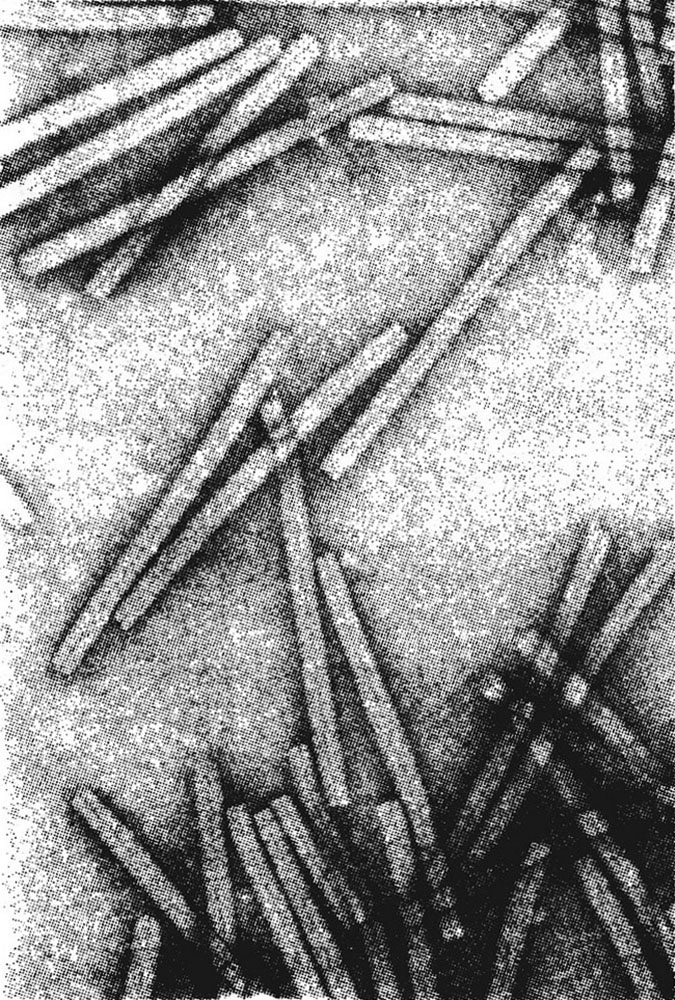
\includegraphics[height=.45\textheight]{img_079.jpg}
\caption[烟草花叶病毒。]
  {烟草花叶病毒。[选自莱宁格[A.Leninger].《生物化学》[\bn{Biochemistry}],纽约:Worth Publishers,1976年版。] }
\end{figure}

\item[阿基里斯]生癌吗?

\item[螃蟹]不,不完全一样,而是——

\item[阿基里斯]难道烟草自己吸烟,得了癌症?正好!

\item[螃蟹]我看你太着急下结论了。阿基。烟草不吸这些“卷烟”。是那些脏乎乎的小“卷烟”来进攻它们,不请自来。

\item[阿基里斯]我明白了。嗯,我现在知道烟草花叶病毒是怎么回事了。那么核糖体呢?

\item[螃蟹]核糖体显然是一种细胞里的东西,可以把某一形式的信息转换成另一种形式的信息。

\item[阿基里斯]有点像微型录音机或唱机什么的,是吗?

\item[螃蟹]作为比喻来说是像。让我感兴趣的是有个活宝在一句话里提到了这样一个事实:同烟草花叶病毒和其它一些稀奇古怪的生物结构一样,核糖体也具有“自发地自组装”这种不可思议的能力。这就是那家伙的原话。

\item[阿基里斯]这是他那些鬼话里的一句,是吧。

\item[螃蟹]这也正是那篇对话里另一个角色的看法。不过这是对那句话的蠢解释。

\dnote{(螃蟹又往烟斗里添了一点稻草末,然后深吸了几口烟斗,一口口地把烟喷到空气中。)}

\item[阿基里斯]嗯,“自发地自组装”是什么意思?

\item[螃蟹]意思是当某个位于细胞内的生物单位分解时,它们可以自发地把它们自己再组装起来——用不着被别的单位来控制。那些部分只要凑在一起——疾!——就粘在一块儿了。

\item[阿基里斯]像魔术似的。要是普通型号的唱机也有这种本事该多好!我是说,既然一部像核糖体这样的微型“唱机”能有这种功能,为什么大一点儿的就不行呢?这样你就能制造出一架不能被摧毁的唱机了,对吗?无论什么时候它被拆散,都能再自行组合起来。

\item[螃蟹]我正是这么想的。我急不可耐地给我的制造商写了一封信,向他解释了自组装的设想,问他能不能给我制造一架可以自行拆散,并能够自发地组装成另一种形式的唱机。

\item[阿基里斯]造这么一个玩艺可太劳神了!

\item[螃蟹]的确,主要是太劳财神了,因为几个月以后,他写信时不仅告诉我他终于成功了,还送来了一张金额巨大的帐单。在这样一个好天里,嘿!我那了不起的自组装唱机终于寄来啦,我信心十足地给龟兄打电话,邀他过来检验检验我这完备的唱机。

\item[阿基里斯]我们眼前这台大家伙一定就是你说的那台吧。

\item[螃蟹]恐怕不是,阿基。

\item[阿基里斯]是不是它又给——

\item[螃蟹]我的老朋友,你所担心的正是事实。我不知道事情是如何发生的。描述当时的情景真太叫人伤心了。眼巴巴地瞧着电线啦、碎片啦乱七八糟地摊了一地,还这儿一股那儿一股地冒着烟——啊,我——

\item[阿基里斯]啊,啊,老蟹,别太想不开。

\item[螃蟹]我倒没什么,只是这一次次的太快了。哼,龟兄开始还幸灾乐祸,最后他看我是真伤心了,于是就同情起我来了。他为了安慰我,就解释说这是理应如此的事,谁也没办法——说这跟什么人的什么“定理”有关,不过那定理我一个字也记不得了,只记得好像叫什么“疙瘩定理”。

\item[阿基里斯]我怀疑这就是他以前跟我说起过的“哥德尔定理”……是有那么点不祥的色彩。

\item[螃蟹]也许吧,我记不起了。

\item[阿基里斯]我向你保证,老蟹,我听你这个故事时是非常同情你的处境的。真太叫人伤心了。不过,你提到过什么稻草的事,请跟我说说,是怎么回事?

\item[螃蟹]噢,对——是有根救命稻草。嗯,我最后终于放弃了寻求“完备的”唱机的念头,而是决定进一步完善对乌龟的唱片的抵制。我抛开了那种能播放一切唱片的唱机的奢望,而是想要一种能避免破坏、能够保存下来的唱机:一种能避免被摧毁的唱机——即使这意味着它只能播放少数一些特殊的唱片。

\item[阿基里斯]于是你就决定以牺牲掉能重现所有可能的声响这一功能为代价,制造一种复杂的反乌龟的机器,对吗?

\item[螃蟹]嗯……说不上我“决定”。更严格地说,是我被迫如此。

\item[阿基里斯]对,我明白你的意思。

\item[螃蟹]我的新设想是不让任何“异己的”唱片在我的唱机上播放。我知道我自己的唱片是不会对我的机器有损害的,所以如果我不让别的唱片混进来,我就能保住我的唱机,用它来欣赏我灌制的唱片。

\item[阿基里斯]这一策略对你的目标很合适。我们眼前这个庞然大物就是你刚才说的那种想法的产物吧?

\item[螃蟹]是的。龟兄自然也认识到他也必须改变策略。他现在的主要目的就是要搞出一种能混过我的检查的唱片来——这是种新挑战啊!

\item[阿基里斯]作为你,你打算怎么排除他或别人的“异己的”唱片呢?

\item[螃蟹]你保证不把我的计划透露给龟兄吗?

\item[阿基里斯]以龟格担保。

\item[螃蟹]什么?

\item[阿基里斯]哦——别担心,这是我从龟兄那儿学来的话——我发誓坚守秘密。

\item[螃蟹]那好吧。我的基本方案是使用标识技术。我的每一张唱片上都有一个秘密标记。现在你面前的这台唱机跟以前那几台一样,都装有一部检验唱片的电视摄像机,这种检验器上配有一台计算机,负责处理那些由检验得到的数据,并控制相应的操作。我打算嚼碎那些没有正确标记的唱片。

\item[阿基里斯]哈,报复他一下!不过我觉得你的方案很容易被挫败。龟兄只要搞到一张你的唱片,复制下那标记,你就没咒念了。

\item[螃蟹]没那么简单,阿基。谁告诉你他能从唱片的非播放状态中知道那个标记的?事情比你想的要复杂哩。

\item[阿基里斯]你是不是说标记跟播放出的音乐是掺在一起的?

\item[螃蟹]正是。但是有办法把它们分解开。这需要从视觉上将那种数据从唱片中抽取出来,然后——

\item[阿基里斯]那种明亮的绿光就是干这个用的,是吗?

\item[螃蟹]对。那是电视摄像机在检查音纹。音纹格式被送到微型电脑里,由它来分析我放进去的唱片的音乐风格——这一切都是无声地进行的。这时不播放唱片。

\item[阿基里斯]是不是有一个甄别过程,将风格不合适的唱片排除掉?

\item[螃蟹]你说对了,阿基。能通过这第二道检查的唱片就只有同我那些唱片风格一样的唱片了——龟兄要摹仿这些简直就是不可能的。所以我坚信我一定能打赢这场新的音乐战。不过,我得说龟兄也同样相信他会混过我的检查。

\item[阿基里斯]最后把这巨大的机器震成碎片?

\item[螃蟹]哦——不,这种结局他已经用事实验证过了。他现在只是想证明不管我采取什么措施,他都能——用一张对我的唱机无害的唱片——溜过我的检查。我听他嘴里不停地嘀嘀咕咕,总是提到一首歌曲,那歌曲的名字挺古怪,叫什么“我可以在唱机X上被播放”。可他吓唬不了我!唯一叫我有些担心的是他似乎同以前一样,又有些什么晦涩的观点,那些观点……\dlnote{(他陷入沉默,随后,满脸沉思的吸了几口烟斗。)}

\item[阿基里斯]哼……我看龟兄那方面有无法克服的困难。他终于碰到对手了!

\item[螃蟹]原来你也这么想……我想你不知道汉肯定理的来龙去脉吧!

\item[阿基里斯]知道谁的定理的来龙去脉?我从没听到过这类事。我相信那一定很吸引人,可我更想多听一些有关“唱片设法混入唱机”的事。这小故事引人入胜呐。其实我都可以说出结局了。显然,龟兄没有找出混进去的突破口,于是只好乖乖认输,就这么回事,不是吗?

\item[螃蟹]至少我是希望这样。你想看看我这台防御式唱机的内部情况吗?

\item[阿基里斯]当然想。我一直想瞧瞧那架电视摄像机。

\item[螃蟹]说干就干,老朋友。\dlnote{(把手伸进那台巨大的唱机张着的“大嘴”里,揿下两个按钮,拿出一台包装整齐的仪器。)}瞧,整个仪器是由一个个独立的模块组成的,可以分别卸下来独立使用。比如这部电视摄像机就能良好地独立工作。看着那边的屏幕,画有燃烧的大号的那幅画下面的那个屏幕。\dlnote{(他将摄像机对着阿基里斯,阿基里斯的脸立刻出现在大屏幕上。)}

\item[阿基里斯]天哪!我可以试试吗?

\item[螃蟹]当然可以。

\item[阿基里斯]\dlnote{(将摄像机对着螃蟹)}你上屏幕了,老蟹。

\item[螃蟹]是啊。

\item[阿基里斯]我要把摄像机对着画有燃烧的大号的那幅画。它现在也在屏幕上啦!

\begin{figure}
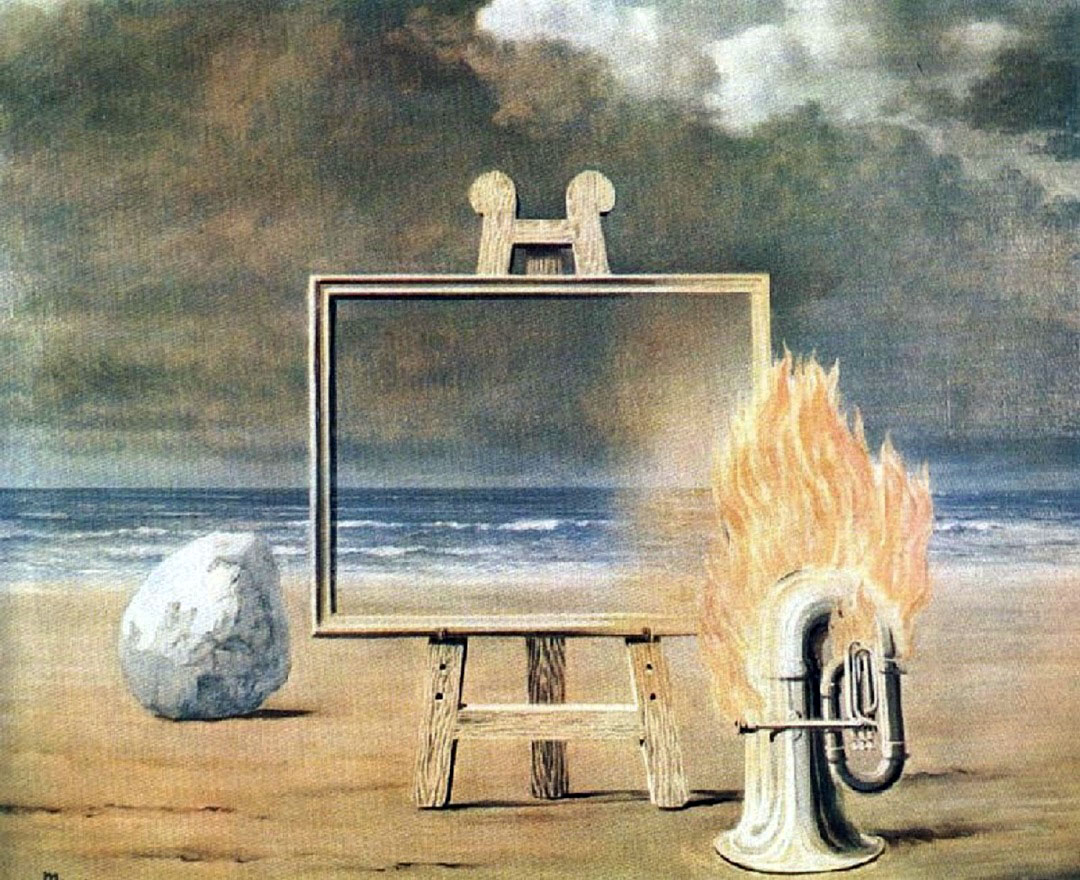
\includegraphics{img_080.jpg}
\caption[漂亮的俘虏,马格里特作。]
  {漂亮的俘虏,马格里特作(1947)。}
\end{figure}

\item[螃蟹]摄像机可以移近移远,阿基。你试试。

\item[阿基里斯]太妙了!让我先对准那些紧挨着画框的火焰……真是不可思议,它能在屏幕上瞬间“复制”出屋里的任何东西——任何我想摄进的东西。我只须把摄像机对准它,像变魔术一样,它立刻就会跳上屏幕。

\item[螃蟹]屋里的任何东西吗,阿基?

\item[阿基里斯]只要是看得见的任何东西,很显然。

\item[螃蟹]要是你把摄像机对准电视屏幕上的火焰,那会怎么样?

\dnote{(阿基里斯调转摄像机,用它对准正播放有火焰的电视屏幕。)}

\item[阿基里斯]太有趣了!这样一来火焰就从屏幕上消失了!它们哪儿去了?

\item[螃蟹]你无法在移动了摄像机时还让屏幕上保持原来的形象。

\item[阿基里斯]我明白了……可我一点也看不懂现在屏幕上是什么!它看上去像一条长长的奇怪的走廊。可我没有把摄像机对着什么走廊啊?我只是把它对着一个普通的电视屏幕。

\item[螃蟹]看仔细些,阿基。你真的看到一条走廊吗?

\item[阿基里斯]啊哈,我现在明白了。那是一组叠套在一起的电视屏幕,一个比一个小……没错儿!火焰的形象早没了,因为我的摄像机不再指向那幅画了。当我把摄像机对着屏幕时,屏幕上就出现了屏幕,包含着屏幕的屏幕上有什么,被包含的屏幕上也就有什么——而被包含的屏幕上只有屏幕,因此被包含的屏幕上有什么,被被包含的屏幕所包含的屏幕上也就有什么——而被被包含的屏幕所包含的屏幕上只有屏幕,因此——

\begin{figure}%
%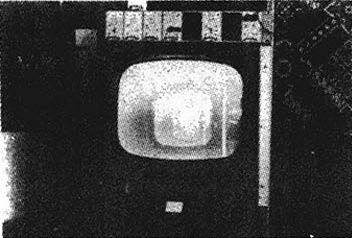
\includegraphics{img_081a.jpg}
\floatsetup{heightadjust=none}
\figurebox[\linewidth]{%
\begin{subfloatrow}[3]
\figurebox{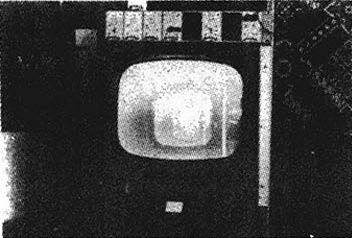
\includegraphics{img_081a.jpg}}
          {\caption{最简单的情形。}}
\figurebox{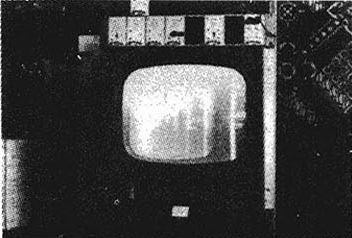
\includegraphics{img_081b.jpg}}
          {\caption{阿基里斯的“走廊”。}}
\figurebox{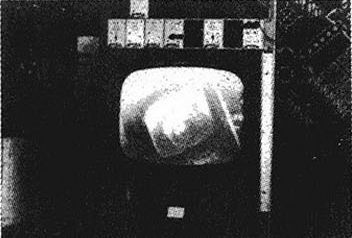
\includegraphics{img_081c.jpg}}
          {\caption{旋转摄像机的情形。}}
\end{subfloatrow}
\par\bigskip
\begin{subfloatrow}[3]
\figurebox{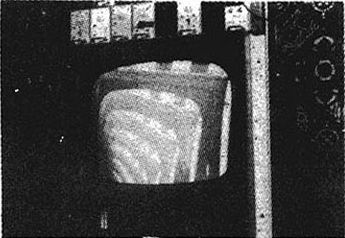
\includegraphics{img_081d.jpg}}
          {\caption{不成功的“自噬”}}
\figurebox{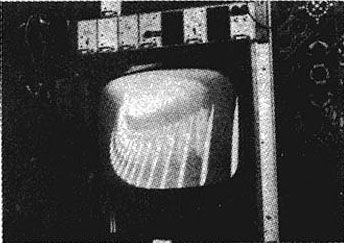
\includegraphics{img_081e.jpg}}
          {\caption{移近时的情形。}}
\figurebox{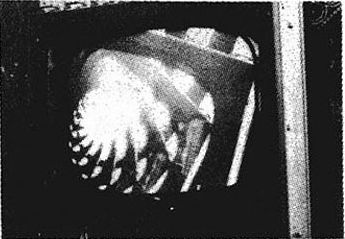
\includegraphics{img_081f.jpg}}
          {\caption{既转动又移拉时的情形。}}
\end{subfloatrow}
\par\bigskip
\begin{subfloatrow}[3]
\figurebox{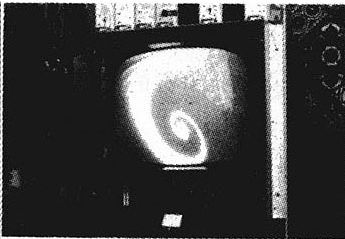
\includegraphics{img_081g.jpg}}
          {\caption{开始变得奇怪起来……}}
\figurebox{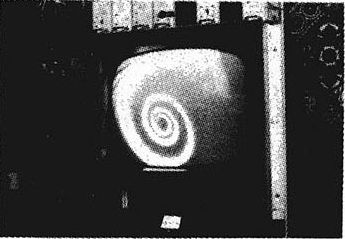
\includegraphics{img_081h.jpg}}
          {\caption{“星系”出现了。}}
\figurebox{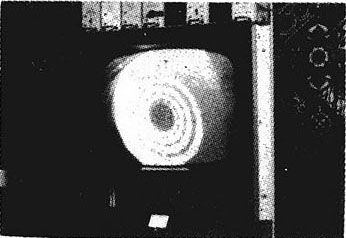
\includegraphics{img_081i.jpg}}
          {\caption{星系在演化……}}
\end{subfloatrow}
\par\bigskip
\begin{subfloatrow}[3]
\figurebox{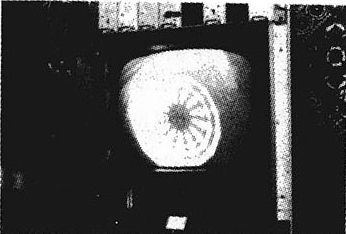
\includegraphics{img_081j.jpg}}
          {\caption{星系的晚期,请数数辐条数。}}
\figurebox{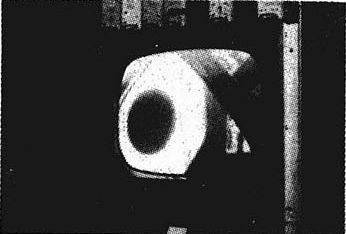
\includegraphics{img_081k.jpg}}
          {\caption{星系把自己烧没了,变成了——一个黑洞!}}
\figurebox{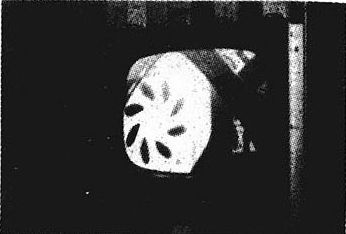
\includegraphics{img_081l.jpg}}
          {\caption{一种“跳动着的花瓣状图像”,摄像时“花瓣”正在移动。}}
\end{subfloatrow}}{%
\caption[自噬的电视屏幕。]
  {十二个自噬的电视屏幕。如果13不是个素数的话,我会再加上二个的。}}
\end{figure}

\item[螃蟹]我想我也能顺着说下去了,阿基。你干嘛不试试旋转旋转摄像机?

\item[阿基里斯]哦!我得到了一根螺旋的走廊!每个屏幕都与它的外框屏幕拧成一定角度,屏幕越小,与最外面的屏幕拧的角度就越大。这种让电视屏幕“自噬”的想法太奇特了。

\item[螃蟹]你说的“自噬”一词是什么意思,阿基?

\item[阿基里斯]我用“自噬”一词是指我把摄像机对准屏幕——或对准屏幕的一部分这一操作,这就是“自噬”,也就是自己吞掉自己。

\item[螃蟹]要是我要求你再说得详细点,你不会不同意吧。我有点叫这个概念给迷住了。

\item[阿基里斯]我也一样。

\item[螃蟹]那好吧。要是你把摄像机对准屏幕的一角,那还算是你说的“自噬”吗?

\item[阿基里斯]让我试试看。哎——屏幕的走廊好像跑到外边去了。这下就没有无穷的叠套了。它挺好看的,可我觉得它不具备“自噬”的因素。它是一种“不成功的自噬”。

\item[螃蟹]要是你把电视摄像机转回屏幕的中心部位,也许你又能把它定住了……

\item[阿基里斯]\dlnote{(小心而缓慢地转动摄像机)}对!走廊变得越来越长啦……瞧啊,完全变回来啦。顺着它一直看下去,能看到它在远处消失了。当摄像机整个儿摄进屏幕时,走廊就又变成无限的了。嗯——这叫我想起不久前龟兄对我说,一个句子要是谈论整个自己,就会出现自指……

\item[螃蟹]什么?请再说一遍。

\item[阿基里斯]没什么——我是在自言自语。

\dnote{(当阿基里斯摆弄起摄像机的镜头和其它控制装置时,屏幕上就出现了前所未有的,花样繁多的“自噬”图像:形似星系的旋转螺线,变化万端的花状图形和其它一些各式各样的图形……)}

\item[螃蟹]你好像玩得挺起劲儿。

\item[阿基里斯\dlnote{(从摄像机那儿转回身来)}]是的!这么一个简单的办法能弄出多少图像啊!\dlnote{(他又转回头盯着屏幕,脸上掠过一丝惊诧的神情。)}哎呀,老蟹!屏幕上出现了一种跳动的花瓣状图形!这种跳动是怎么产生的?电视机是静止的,摄像机也没动呀。

\item[螃蟹]偶尔你也可以弄出些在时间中有变化的图形。这是由于在摄像机“看到”什么东西和把它显示在屏幕上这两者之间时间上稍有先后之差,这是由线路造成的,这个时间差大约是百分之一秒。所以要是你弄出一个由五十个环像组成的套叠,其时间差大约就要有半秒。要是把某种活动的东西弄进屏幕——比方说,把你的手指放到摄像机前,那么,就得过一会儿才能在套得更深一些的屏幕上“把它找出来”。这种时间延宕反映到整个系统,就形成了某种视觉“回声”。如果创造出一种条件,使得这种回声不消逝,就会形成跳动的图形。

\item[阿基里斯]太了不起啦!你说,要是我们试试弄出一个全自噬会怎么样?

\item[螃蟹]你是什么意思?说得明白些。

\item[阿基里斯]嗯,我是觉得这种屏幕里面有屏幕的东西非常有趣,可我更想得到一幅里面有这部电视摄像机以及这个屏幕的图像,让它显现到这个屏幕上。那样我才能真正使一个系统自噬其自身。因为这个屏幕仅仅是这整个系统的一部分。

\item[螃蟹]我明白你的意思了。也许你能利用镜子获得你所要的效果。

\dnote{(螃蟹递给他一面镜子,阿基里斯操纵镜子和摄像机,使得摄像机和屏幕都显现在屏幕上。)}

\item[阿基里斯]瞧!我创造出了完全的自噬!

\item[螃蟹]我觉得只有镜子的前面还不够,加上它的背面怎么样?要是没镜子背面,那它就不能反射——你就没法儿使图像里也有摄像机了。

\item[阿基里斯]你说的对。不过,要既显出镜子的正面,也显出背面,我就不得不再需要一面镜子。

\item[螃蟹]可你还得显出第二面镜子的背面。除了显示摄像机的前面以外,把它的背面也弄进去怎么样?还有电源线,还有电视内部,还有——

\item[阿基里斯]哎哟哟!我的脑袋都晕了!看来我这个“全自噬计划”要出麻烦了。我现在觉得昏昏然的。

\item[螃蟹]我能体会到你这时的感觉,你干嘛不坐下来,抛开这些什么鬼自噬?放松放松!看看我的画你就会平静下来的。

\dnote{(阿基里斯唉声叹气地躺下了。)}

哦——也许我的烟味叫你不舒服?得,我拿开它。\dlnote{(把烟斗从嘴上拿掉,小心地放在马格里特的另一幅画里面的一句话的上方。)}喏,好些了吧?

\item[阿基里斯]还是恶心。\dlnote{(指着马格里特的画。)}这幅画挺有意思,我喜欢它的外框,很有质感。

\begin{figure}
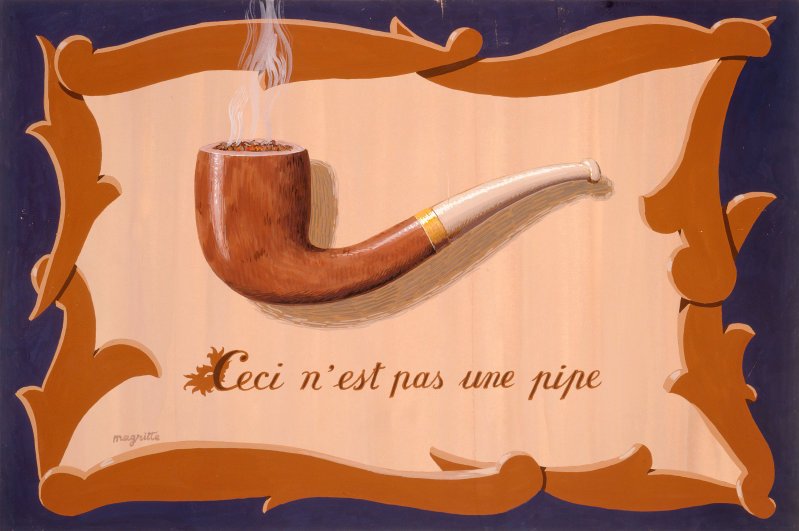
\includegraphics{img_082.jpg}
\caption[咏叹调和歌曲,马格里特作。]
  {咏叹调和歌曲,马格里特作(1964)。}
\end{figure}

\item[螃蟹]谢谢。那是我特地请人做的——用烟叶和稻草。

\item[阿基里斯]用烟叶和稻草?乖乖,真叫人难以相信!烟斗下面写的是什么字?不像英文,是吧?

\item[螃蟹]是法文。写的是“Ceci n'est pas une pipe.”,意思是“这不是一只烟斗”。千真万确。

\item[阿基里斯]可它是一只烟斗啊!你刚才还吸来着!

\item[螃蟹]哦,我想你误解了这句话的意思。“ceci”这个词指那幅画,而不是指烟斗。烟斗当然是烟斗,可一幅画却不是一只烟斗。

\item[阿基里斯]我不知道画中的“ceci”一词是指整幅画,还是指画中的烟斗。哦,我的天!这又是一个自噬!我可真不行了,老蟹,我想我快要病了……

\end{dialogue}

\end{dialog}
